\section{Fundamentals}
\label{sec:fundamentals}

\subsection{Distributed Array Computation}
\label{ssec:distributed_array_computation}
General array computation is used in a lof of scientific fields nowadays.
Simulation of atomic levels or measurements of fuel are fine grained enough to have huge data amounts
and they still need to be processed.
One elegant way to solve this is the use of distributed computing. By using multiple machines at once
the computing time should go down while the available memory increases.
But writing distributed programs from scratch is hard problem especially for scientists that have limited amount
of experience with computing in comparison to computer scientists.


\subsection{HEAT}
\label{ssec:heat}
\gls{HeAT} is introduced in \cite{krajsek_helmholtz_nodate}. HeAT aims to be a mathemtical library for distributed computations.
It conforms to a Numpy \cite{noauthor_numpy_nodate} interface and make all distributed calculations transparent. To move from executing \gls{HeAT} scripts to executing them parallel
or distributed one just needs to change the execution command to MPI.
This is due to \gls{HeAT} wrapping PyTorch as implementation with the correct \gls{MPI} synchronization to distribute the calculation.

To perform the calculation distributed correctly \gls{HeAT} adds a new data structure: the DNDArray. Users of other libraries
recognize the general interface of Numpy arrays or PyTorch Tensors, but extended by a split parameter.
The split parameter allows to control the axis, which \gls{HeAT} distributed across the different nodes.

Although, the distribution is transparent besides the split parameter, several pitfalls exist.
When reshaping or splicing the dataset one has to potentially rebalance the dataset. Additionally, this could incurr communication effort
to redistribute the dataset across the nodes.
Another pitfalls especially for developers comming from the distributed programming, lies in all processes needing to call all \gls{HeAT} methods.
While in traditional \gls{MPI} one discriminates between the processes based on the rank, in \gls{HeAT} all nodes need to access all functions and DNDArrays or the
programm could lockup.

Lastly, \gls{HeAT} provides the load utility for distributed loading of datasets. Through the usage of all nodes at the same time IO is maximized and the data
is splitted already during loading. Therefore, calculations can start right away without the need to distribute the data.
\cite{krajsek_helmholtz_nodate}


\subsection{Local Climate Zone Classification}
\label{ssec:local_climate_zone_classification}

\begin{figure*}[t]
  \centering
  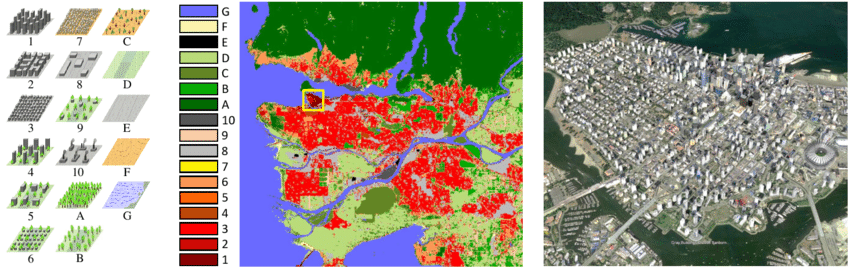
\includegraphics[width=0.9\linewidth]{images/schematic-lcz.png}
  \caption{The LCZ classes as schematics on the left and matching of classes for a city in the centre. Image taken from \cite{zhu_so2sat_2019}.}\label{fig:lcz_classes}
\end{figure*}

\gls{LCZ}s are a scheme formally proposed by \citeauthor{stewart_local_2012} in \cite{stewart_local_2012}. The scheme classifies areas based on fabric, land cover, structure
and metabolism into one of 17 \gls{LCZ}s. \cite{xue_applications_2020}
The \gls{LCZ}s are decided by 4 components:
\begin{enumerate}
  \item Height of roughness features
  \item Packing of roughness features
  \item Surface cover around roughness features
  \item Thermal admittance of materials
\end{enumerate}
The different classes can be seen in figure \ref{fig:lcz_classes}.



\subsection{SO2Sat}
\citeauthor{zhu_so2sat_2019} presented the SO2Sat dataset in \cite{zhu_so2sat_2019}. They describe SO2Sat as a \enquote{valuable benchmark dataset [...], which consists of local climate zone (LCZ) labels of about half a million [...] image patches}.
These images are taken from Sentinel-1 and Sentinel-2. Each image is 32 by 32 pixels and contains 8 channels for Sentinel-1 and 10 channels for Sentinel-2.
After preprocessing these images they were given to domain experts for labelling which follwed a \enquote{carefully designed labelling work flow}.
Through the careful work the dataset achieved a \enquote{overall confidence of 85\%}.
The annotations contains the 17 LCZ classes.
The regions of the dataset are 52 cities.

\subsection{Spectral Clustering}
\label{ssec:spectral_clustering}

\begin{algorithm}[h]
  \SetKwData{Laplace}{\(L\)}\SetKwData{Adj}{\(W\)}
  \KwData{Similariy matrix \(S\), number \(k\) of clusters}
  \KwResult{Clusters \(A_1, \ldots, A_k\) }
  Construct a similarity graph\;
  \Adj \(\leftarrow\) weighted adjacency matrix\;
  \Laplace \(\leftarrow\) computeLaplacian(\Adj)\;
  \(u_1, \ldots, u_k \leftarrow\) computeEigenvectors(L)\;
  \(U\) \(\leftarrow\) Matrix with columns \(u_1, \ldots, u_k\)\;
  \ForEach(){\(i = 1, \ldots, n\)}{
    \(y_i\) \(\leftarrow\) vector corresponding to the \(i\)-th row of \(U\)
  }
\(C_1, \ldots, C_k \leftarrow\) kMeans(\(y_1, \ldots, y_n\))\;

  \caption{Basic Spectral Clustering}\label{alg:basic_spectral}
 \end{algorithm}

\enquote{Spectral Clustering is the process of partitioning data samples into
\(k\) groups based on graph theory} \cite{krajsek_helmholtz_nodate}. Therefore,
to derive the formulation of Spectral Clustering we introduce the undirected graph \(G=(V, E)\).
We consider the graph as weighted by assigning each edge an weight \(w_{ij}\). As the graph
is unidrectional, the weight is identical for \(w_{ij} = w_{ji} \).
% Degree Matrix
We define the degree of a vertex \(v_i \in V\) by iterating over all vertices \(v_j \in V\) that are connected to \(v_i\).
Therefore, the weight of the edge is positive:
\[d_i = \sum_{j=1}^n w_{ij}\]
Using the degree defined before, we define the degree matrix \(D\) as the diagonal matrix whith the degrees \(d_1, \ldots, d_n\) on the diagonal.
\cite{von_luxburg_tutorial_2007}
% Weights Matrix
For 2 subsets of indices \(A, B\) we define the weights matrix \cite{von_luxburg_tutorial_2007}:
\[W(A, B) := \sum_{i \in A, j \in B} w_{ij}\]


There are several possible ways to construct such a similarity graph from two datasets.
The following three are used often for spectral clustering:
\begin{itemize}
  \item Fully connected
  \item Symmetric
  \item \(\epsilon\)-Neighbourhood
\end{itemize}
According to \cite{von_luxburg_tutorial_2007} there is no theoretical work on the choosing of one method over
another.

Using the constructed similarity graph we need to calculate the spectrum of the similarity matrix.
This is done by constructing the Laplacian defined via
\[L = W - D\]
using \(W, D\) as defined earlier.

The Lanczos algorithm \cite{lanczos_iteration_1950} is used to calculate the eigenvalues and eigenvectors from the laplacian.
When using the \(k\) smallest eigenvalues and the korresponding eigenvectors \(e_1, \ldots, e_k\) we can embedd the dataset.

Now a clustering can be performed in the smaller embedding space of the eigenbasis using another algorithm, e.g. KMeans.
The overall algorithm can be found in algorithm \ref{alg:basic_spectral}.


\subsection{Clustering Evaluation Metrics}
\label{ssec:clustering_evaluation_metrics}

Evaluating clusters is more complicated than evaluating classification or other supervised machine learning tasks.
Unsupervised tasks can be evaluating using interal or external metrics. While, internal metrics are derived from the algorithm itself e.g. Cluster purity, external metrics need labels for the dataset.

Due to in this work used dataset having labels, this section is going to focus on external metrics.
For the here presented metrics we define \(C\) as the ground truth classes and \(K\) as the clustering assignment.
ON this basis we define the following:\\
\(a\) - the number of pairs of elements that are in the same set in \(C\) and in the same set in \(K\)\\
\(b\) - the number of pairs of elements that are in different sets in \(C\) and in different sets in \(K\)\\


\subsubsection{Adjusted Rand Index}
The \gls{ARI} measures the similarity of two assignments. While the raw Rand Index has problems with random assignments, the \gls{ARI} assigns a score close to \(0\)
to random assignments.
The raw Rand Index is mathematically given by \cite{noauthor_23_2020} as
\[RI = \frac{a + b}{C_2^{n_{samples}}}\]
When adjusting this index for random assignments we yield:
\[ARI = \frac{RI - \mathbb{E} [RI]}{\max (RI) - \mathbb{E} [RI]}\]
